\chapter{The \chips R\&D Project} %%%%%%%%%%%%%%%%%%%%%%%%%%%%%%%%%%%%%%%%%%%%%%%%%%%%%%%%%%%%%%%%
\label{chap:chips}

In pursuit of answers to the open questions outlined in the previous chapter, neutrino experiments
are becoming increasingly, and possibly prohibitively, expensive and impractical. This is
particularly true of the next generation of long baseline experiments, DUNE and Hyper-Kamiokande,
with cost estimates reaching billions of dollars and construction times greater than half a decade
long. It is also telling that these two future experimental neutrino projects receive the vast
majority of global research effort, such is their complexity, cost, and lead time.

It is clear that for detectors to remain practical and affordable into the future, a novel
approach to neutrino detector design is highly desirable. This is especially the case if megaton
scale detectors are ever to become a reality. While instrumentation will continue to improve with
time, the statistics of low event counts will always limit neutrino experiments until vastly
larger detectors can be built. Therefore, current R\&D efforts must focus on such detectors while
also attempting to complement the current and upcoming generation of experiments.

The \chips R\&D project~\cite{adamson2013} aims to develop novel strategies and technologies for
very large yet `cheap as chips' water Cherenkov detectors. Primarily aimed for deployment in long
baseline accelerator beam scenarios, \chips aims to lower the construction cost per kt of fiducial
mass to between \$200k-\$300k. For comparison, the Super-Kamiokande detector reached a cost of
approximately \$4 million/kt to build. As physics sensitivity depends on more than just fiducial
volume, this comparison is not entirely rigorous; however, it highlights the scale of cost savings
possible.

This chapter aims to describe the fundamental aspects of the \chips R\&D project in detail.
Firstly, the \chips concept will be outlined along with neutrino beam and Cherenkov detector
physics for context. The design, construction, deployment, and status of the \chipsfive detector
will then follow. Finally, the Monte Carlo event generation and detector simulation framework will
be discussed to aid the discussion of work presented in later chapters of this thesis.

\section{\chips concept} %%%%%%%%%%%%%%%%%%%%%%%%%%%%%%%%%%%%%%%%%%%%%%%%%%%%%%%%%%%%%%%%%%%%%%%%%
\label{sec:chips_concept} %%%%%%%%%%%%%%%%%%%%%%%%%%%%%%%%%%%%%%%%%%%%%%%%%%%%%%%%%%%%%%%%%%%%%%%%

The \chips concept is to construct cylindrical water Cherenkov detectors that can be sunk to the
bottom of deep bodies of water on the Earth's surface, such as lakes, reservoirs and flooded mine
pits. The water above the sunken detector provides a modest overburden from cosmic rays, while the
surrounding water provides support for a lightweight detector structure. By removing the need for
underground excavation and expensive structural support, the cost of construction can be
dramatically reduced.

Additionally, the common practice of building majority bespoke components is replaced by using
modern commercially available components wherever possible. The number of expensive elements, such
as photomultiplier tubes is also reduced by only considering accelerator beam neutrino events,
such that full coverage high-density detector instrumentation is not required.

Furthermore, \chips detectors are not only designed to be cheap but practical. Easy to build,
quick to deploy, and upgradable once operational, multiple detector modules can be flexibly
combined depending on available resources. When compared to DUNE and Hyper-Kamiokande both
requiring a large upfront budget and many years to construct, cheap \chips detector modules can be
flexibly deployed in under a year by a relatively small team.

To date, \chips R\&D efforts have been based in the USA to exploit the NuMI beam before the end of
its lifetime. Future plans are focused on the scaling \chips detectors for the deployment of
multiple modules within the LBNF beam once operational. Collaborators from primarily University
College London, The University of Wisconsin Madison and Nikhef are focused on multiple R\&D
efforts outlined below, each aiming to prove the viability of a crucial component of the \chips
concept.

\begin{itemize}
    \item \textbf{Detector construction:} This effort aims to prove that the construction and
          deployment of \chips concept detectors are possible. Two prototype detectors have so far
          been deployed. Firstly, the small \chipsm detector~\cite{perch2015, pfutznerProto2017,
              pfutzner2017}, deployed into a flooded mine pit located in northern Minnesota during the
          summer of 2014, as shown in Fig.~\ref{fig:chips_m}. Secondly, the much larger
          \unit{5}{\mathrm{kt}} \chipsfive detector, deployed into the same pit during the summer
          of 2019 and detailed in Section.~\ref{sec:chips_detector}.

    \item \textbf{Water filtration:} This effort aims to prove that adequate water purity can be
          achieved using cheap, commercially available filtration. Extensive
          studies~\cite{amat2017, campbell2020} have proven that by filtering water directly from
          bodies of water on the Earth's surface (including flooded mine pits), adequate photon
          attenuation lengths, greater than \unit{50}{\mathrm{m}} are achievable.

    \item \textbf{Detector sensitivity:} This effort aims to prove that \chips concept detectors
          (even prototypes) can provide significant physics contributions alone or alongside the
          current and next generation of experiments. Single detectors in the current NuMI beam
          (discussed in Section.~\ref{sec:chips_concept_beam}) and multiple detectors in the
          future LBNF beam have been considered in multiple studies~\cite{pfutzner2017, adde2016,
              lang2015}.

    \item \textbf{Data acquisition:} This effort aims to prove that a cheap data acquisition
          system using commercially available components and software is viable~\cite{eijk2018}.
          Outlined in Chapter.~\ref{chap:daq}, \chips implements a novel use of cheap single-board
          computers to collect photomultiplier tube data.

    \item \textbf{Event reconstruction and classification:} This effort aims to prove that modern
          machine learning techniques can be successfully applied to large water Cherenkov
          detector concepts such as \chips. Outlined as the primary contribution of this thesis in
          Chapter.~\ref{chap:cvn}, this work feeds directly into both the detector sensitivity
          work mentioned above and detailed detector optimisation studies.
\end{itemize}

\begin{figure} % CHIPS-M DIAGRAM %
    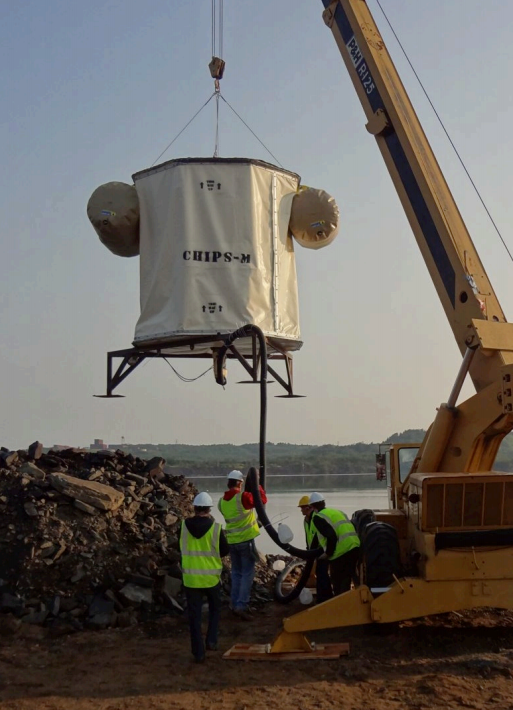
\includegraphics[width=0.6\textwidth]{diagrams/4-chips/chips_m.png}
    \caption[Picture of the \chipsm detector.]
    {Picture of the \chipsm detector just before deployment. The temporary floatation bags are
        visibly attached to the top rim of the detector. Additionally, the umbilical cord carrying
        data, power, and water is attached to the bottom of the detector.}
    \label{fig:chips_m}
\end{figure}

\subsection{The neutrino beam and off-axis alignment} %%%%%%%%%%%%%%%%%%%%%%%%%%%%%%%%%%%%%%%%%%%%
\label{sec:chips_concept_beam} %%%%%%%%%%%%%%%%%%%%%%%%%%%%%%%%%%%%%%%%%%%%%%%%%%%%%%%%%%%%%%%%%%%

\chips detectors will primarily study the appearance of $\nu_{e}$ oscillating from $\nu_{\mu}$
over a long baseline. To generate a sufficient number of GeV scale $\nu_{\mu}$, a high-intensity
accelerator beam is required. Currently, only two such beams exist, the J-PARC based beam in Japan
used by the T2K experiment and the \numi beam in the USA used by \nova. Here we describe the
\numi~\cite{adamson2016} (Neutrinos at the Main Injection) beam as it is directly relevant to
current \chips efforts. However, it is essential to note that \chips detectors are designed to be
used in any neutrino beam, including the future \numi replacement, LBNF.

The \numi beam is an accelerator muon neutrino beam produced at Fermilab near Chicago in the USA.
Beginning operation in 2005 for the MINOS experiment, \numi was upgraded in 2013 to provide a
higher intensity and energy, principally to achieve peak energy near the $\sim$\unit{1.5}{\GeV}
$\nu_{\mu}\rightarrow\nu_{e}$ oscillation maximum for \nova. Currently the \numi beam achieves an
intensity above \unit{700}{\mathrm{kW}} (\unit{740}{\mathrm{kW}} peak) making it the most powerful
beam in the world. A schematic of the \numi beamline configuration is shown in
Fig.~\ref{fig:numi_beam}.

\begin{figure} % NUMI BEAM DIAGRAM %
    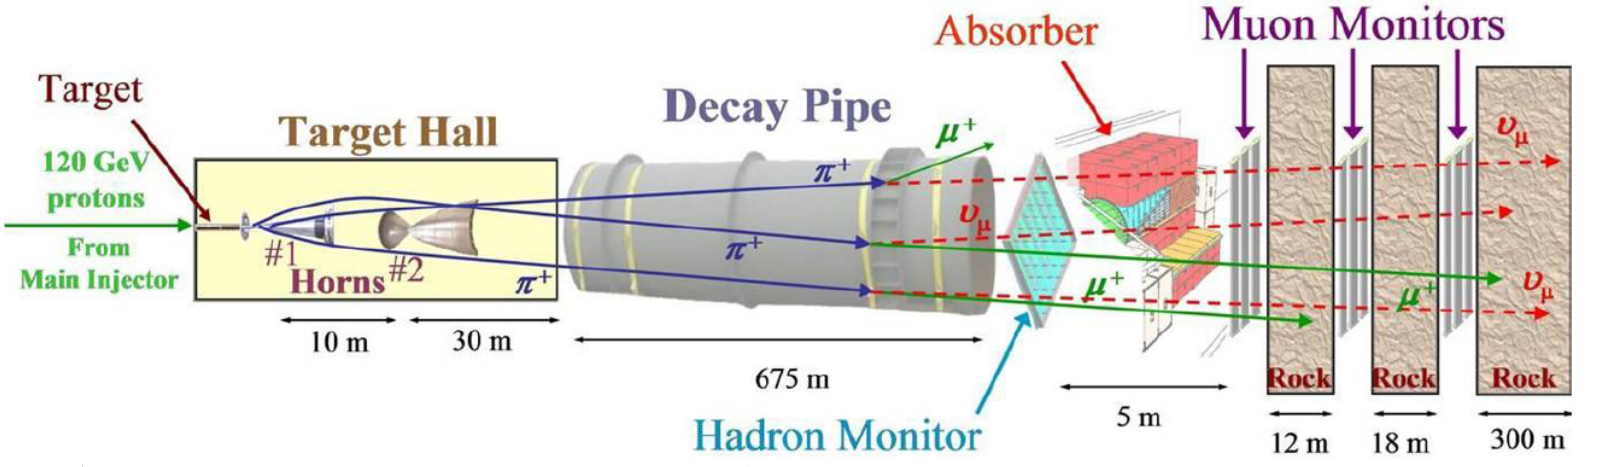
\includegraphics[width=\textwidth]{diagrams/4-chips/numi_beam.png}
    \caption[Schematic of the main components of the \numi beam.]
    {Schematic of the main components of the \numi beam (not to scale) shown with dimensions.
        Figure taken from Ref.~\cite{adamson2016}. The MINOS and \nova near detectors and the
        MINERvA experiment are located just to the right of what is shown.}
    \label{fig:numi_beam}
\end{figure}

Every \unit{1.33}{\mathrm{seconds}} a \unit{10}{\mu\mathrm{s}} long spill of protons accelerated
to \unit{120}{\GeV} by the Main Injector are directed towards a stationary graphite target. The
resulting interactions within the target create a shower of secondary hadrons containing
predominantly pions and kaons. The hadrons are passed through a focusing system of two magnetic
horns tuned principally to focus charged pions along the beamline while rejecting other particles.
After focusing, the surviving hadrons are allowed to decay in flight to a beam of muon neutrinos
in a \unit{675}{\mathrm{m}} long decay pipe via the processes,
\begin{align} % NUMI DECAY EQUATIONS %
    \pi^{+} & \rightarrow\mu^{+}+\nu_{\mu}, \\
    K^{+}   & \rightarrow\mu^{+}+\nu_{\mu}. \\
    \label{eq:numi_decays}
\end{align}
The resulting muons also decay such that $\mu^{+}\rightarrow e^{+}+\nu_{e}+\bar{\nu}_{\mu}$
producing an intrinsic $\nu_{e}$ background (alongside other decays) as well as wrong sign
$\nu_{\mu}$ contamination. Alternatively, the polarity of the horns can be used to switch the
dominant sign of the hadrons focused, allowing \numi to operate as either a neutrino or
antineutrino beam. These two modes of operation are called \emph{forward horn current} and
\emph{reverse horn current} for primarily a neutrino or antineutrino beam composition
respectively. Any remaining hadrons, alongside electrons, muons and surviving primary protons are
absorbed by rock downstream of the decay pipe, leaving just the neutrino components of the beam.

Long baseline neutrino experiments typically consist of a \emph{near detector} to measure the beam
neutrino composition at source and a much larger \emph{far detector} to measure the oscillated
composition after a long distance. The \numi beamline contains three detectors just downstream of
\unit{300}{\mathrm{m}} of rock: The MINERvA spectrometer~\cite{mcfarland2006}, the near detector
for MINOS (now used by MINERvA), and the near detector for \nova. \chips prototypes within the
\numi beam will not have a dedicated near detector; therefore, data from the above detectors will
be crucial for physics analysis in order to constrain the beam composition and flux. However, any
future near detector for \chips, possible in the LBNF beam should also be a water Cherenkov
detector, so that detector induced systematic uncertainties can cancel.

The \numi neutrino beam passes through the Earth's crust until it finally emerges in northern
Minnesota. This is where the MINOS, \nova, and prototype \chips far detectors are located (used to
be located in the MINOS case), as shown in Fig.~\ref{fig:numi_map}. The Minnesota state nickname
`land of 10,000 lakes' is not an overstatement, there are a large number of potential lakes for
\chips detector deployment in this region. Additionally, intense iron ore mining activity on the
`Iron Range' provides many suitable disused (and now flooded) mine pits. The exact \chipsfive
prototype detector location is discussed in greater detail in Section.~\ref{sec:chips_detector}.

\begin{figure} % CHIPS LOCATION IN NUMI DIAGRAM %
    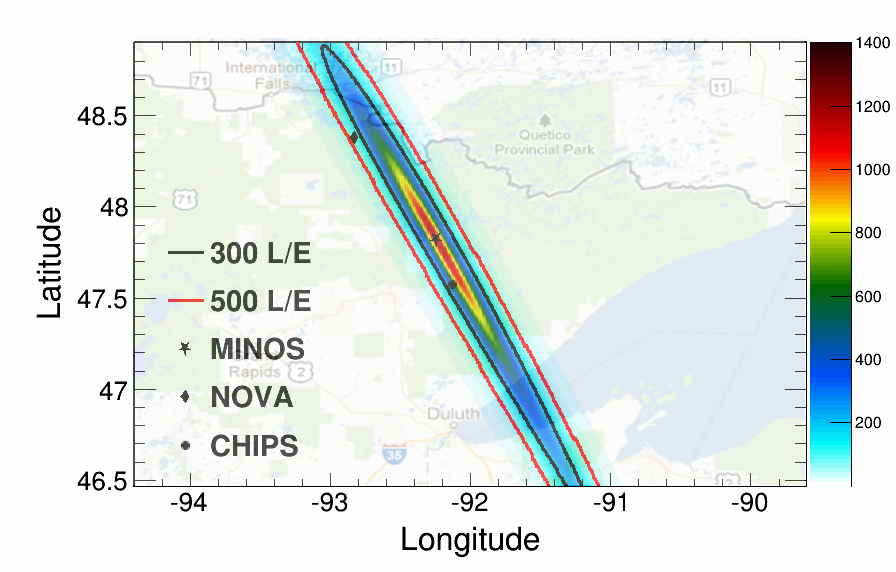
\includegraphics[width=0.7\textwidth]{diagrams/4-chips/numi_map.png}
    \caption[Map of detector locations in the \numi beam.]
    {Map of the MINOS, \nova and \chips locations in the \numi beam as it surfaces in northern
        Minnesota. Shown is the expected neutrino event rate assuming no oscillations, with lines
        of constant L/E indicated by contours. The western extent of Lake Superior can be seen in
        the lower right of the map. Image taken from Ref.\cite{adamson2013}.}
    \label{fig:numi_map}
\end{figure}

Due to the kinematics of pion decay, whether the far detector is placed directly on the beam axis
or not can have a significant impact on the observed energy spectrum of beam neutrinos as shown in
Fig.~\ref{fig:numi_axis}. For neutrinos directly on the beam axis, there is a strong energy
dependence on the parent pion energy. However, as the off-axis angle increases, the neutrino
energy is less dependent on the parent pion energy and becomes restricted to a narrowing range of
decreasing energies. This effect known as the \emph{off-axis effect} is used by both \nova and T2K
to create a narrower energy spectrum focused on the $\nu_{\mu}\rightarrow\nu_{e}$ oscillation
maximum. Additionally, by reducing the tail of higher-energy neutrinos, the number of background
NC events can be greatly reduced, as is the case for the \unit{7}{\mathrm{mrad}} off-axis
\chipsfive detector.

\begin{figure} % OFF-AXIS FLUX DIAGRAM %
    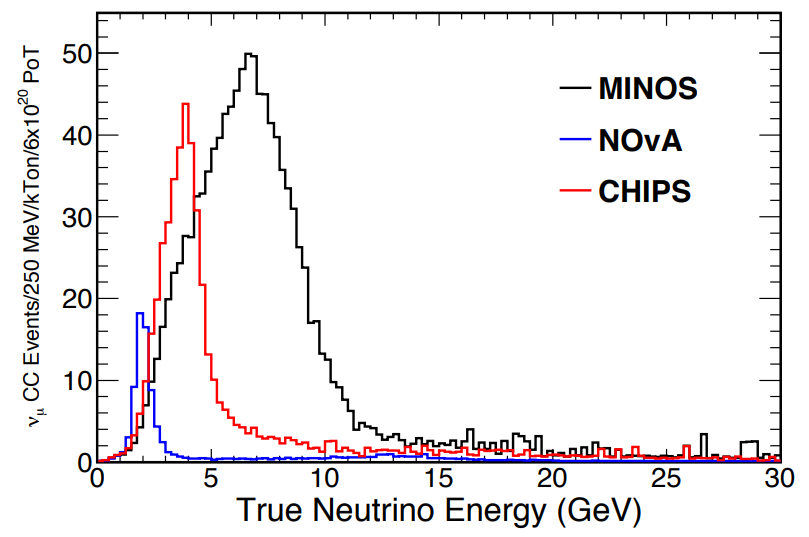
\includegraphics[width=0.6\textwidth]{diagrams/4-chips/numi_axis.png}
    \caption[Muon neutrino flux for different \numi detectors at different off-axis angles.]
    {Muon neutrino flux for different \numi detectors at different off-axis angles. Shown are the
        neutrino energy spectrum for MINOS (on-axis), \nova (\unit{14}{\mathrm{mrad}} off-axis),
        and \chipsfive (\unit{7}{\mathrm{mrad}} off-axis). Figure taken from
        Ref.~\cite{adamson2013}.}
    \label{fig:numi_axis}
\end{figure}

\subsection{Water Cherenkov detectors} %%%%%%%%%%%%%%%%%%%%%%%%%%%%%%%%%%%%%%%%%%%%%%%%%%%%%%%%%%%
\label{sec:chips_concept_cherenkov} %%%%%%%%%%%%%%%%%%%%%%%%%%%%%%%%%%%%%%%%%%%%%%%%%%%%%%%%%%%%%%

The \chips detector concept is based upon the water Cherenkov technique for neutrino detection,
which has successfully been used many times by neutrino experiments. A large body of target water
is instrumented with photomultiplier tubes (PMTs) to record the Cherenkov radiation produced by
sufficiently relativistic charged particles resulting from neutrino interactions. By using readily
available water as the target material and only instrumenting the volume surface, water Cherenkov
detectors provide the best detection methodology for maximising volume and reducing cost.

Cherenkov radiation is emitted by all electrically charged particles travelling faster than the
local phase velocity of light in a dielectric medium. Similar to the sonic boom created by a
supersonic aircraft, Cherenkov radiation forms a shock wave of coherent light, as shown in
Fig.~\ref{fig:cherenkov}, typically with wavelengths in the ultraviolet and optical range. When
projected onto the detector wall, the resulting cone of radiation generates a distinctive ring
shape. The cone opening angle (the angle at which light is emitted) $\theta_{c}$ is given by:
\begin{equation}
    \cos\theta_{c} = \frac{1}{\beta n(\lambda)},
    \label{eq:cherenkov_angle}
\end{equation}
where $\beta=v/c$ and $n$ is the refractive index of the medium~\cite{particle2020}. Note that $n$
is a function of the wavelength of emission $\lambda$, and so is the opening angle. As the
refractive index of water is $\sim 1.33$ for typical wavelengths of emission, and using the
ultrarelativistic limit $\beta\sim 1$ the opening angle is found to be $\sim41^{\circ}$.

\begin{figure} % CHERENKOV EFFECT DIAGRAM DIAGRAM %
    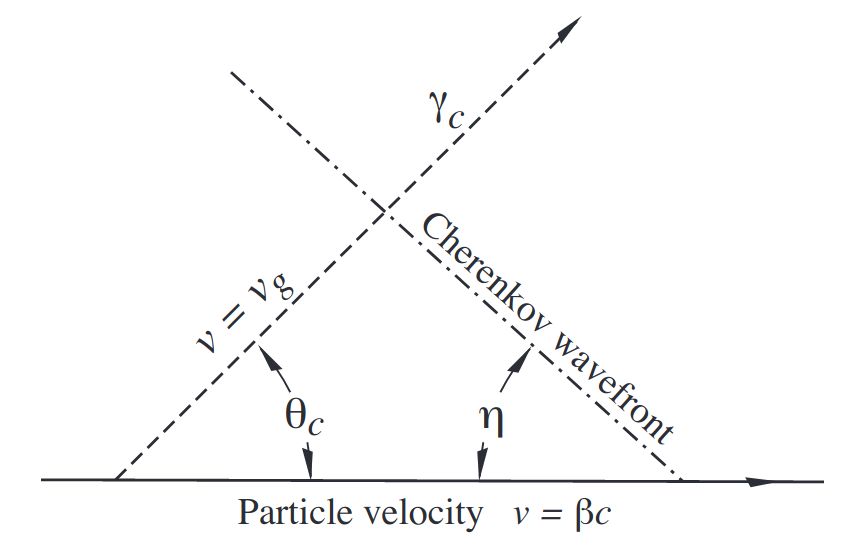
\includegraphics[width=0.6\textwidth]{diagrams/4-chips/cherenkov.png}
    \caption[Diagram of Cherenkov radiation emission.]
    {Diagram of Cherenkov radiation emission and wavefront angles. The angles $\theta_{c}$ and
        $\eta$ are not equal in a dispersive medium. Figure taken from Ref.~\cite{particle2020}}
    \label{fig:cherenkov}
\end{figure}

There is no Cherenkov emission when $\cos\theta_{c} > 1$ in Eq.~\ref{eq:cherenkov_angle}, which is
the case when $\beta n(\lambda)<1$. Therefore, there exists a Cherenkov energy threshold $E_{t}$
for every particle, which when expressed in terms of the particle mass $m$ is given by:
\begin{equation}
    E_{t} = \gamma m = \frac{m}{\sqrt{1-(1/n)^{2}}}.
    \label{eq:cherenkov_threshold}
\end{equation}
Again using $n\sim 1.33$ this gives a typical threshold energy of $\sim1.5m$.

The number of Cherenkov photons emitted by a particle of charge $ze$ per unit wavelength per unit
path length is given by:
\begin{equation}
    \frac{d^{2}N}{d\lambda dx}=\frac{2\pi\alpha z^{2}}{\lambda^{2}}
    \left(1-\frac{1}{1-\beta^{2}n^{2}(\lambda)}\right),
    \label{eq:cherenkov_emission}
\end{equation}
where $\alpha$ is the fine structure constant~\cite{particle2020}. Integrating over the range of
wavelengths for which PMTs are typically sensitive, \unit{350}{\mathrm{nm}} to
\unit{650}{\mathrm{nm}}, and using $\beta\sim 1$ and $n\sim 1.33$ gives approximately $240$
photons emitted per cm travelled by the charged particle~\cite{perch2017}.

By analysing the Cherenkov ring (or rings) of light recorded by the PMTs on the walls of the
detector, information about the charged particle (particles) within an event can be determined.
The underlying neutrino interaction can then be understood indirectly. The primary challenge for
accelerator beam water Cherenkov detectors is the identification and reconstruction of an electron
or muon ring likely to have been produced initially from a beam neutrino and not a cosmic ray.
This indicates a beam CC $\nu_{e}$ or CC $\nu_{\mu}$ event respectively, rejecting NC events.

The basic shape of a Cherenkov ring can be used to tell which charged particle created it
(particle identification). Muons are long-lived and typically travel many metres within the
detector, producing a clean ring with sharp edges. Conversely, electrons almost immediately
initiate an electromagnetic shower; therefore, the observed ring is the sum of all the rings
produced from the individual electrons and positrons within the shower. As a consequence, when
compared to a muon ring, electron rings are commonly wider and characteristically fuzzy and less
sharp. This difference can somewhat be seen in Fig.~\ref{fig:emission distance} which shows how
the total amount of Cherenkov radiation is emitted for both electrons and muons as a function of
distance from the interaction vertex.

\begin{figure} % EMISSION DISTANCE DIAGRAM %
    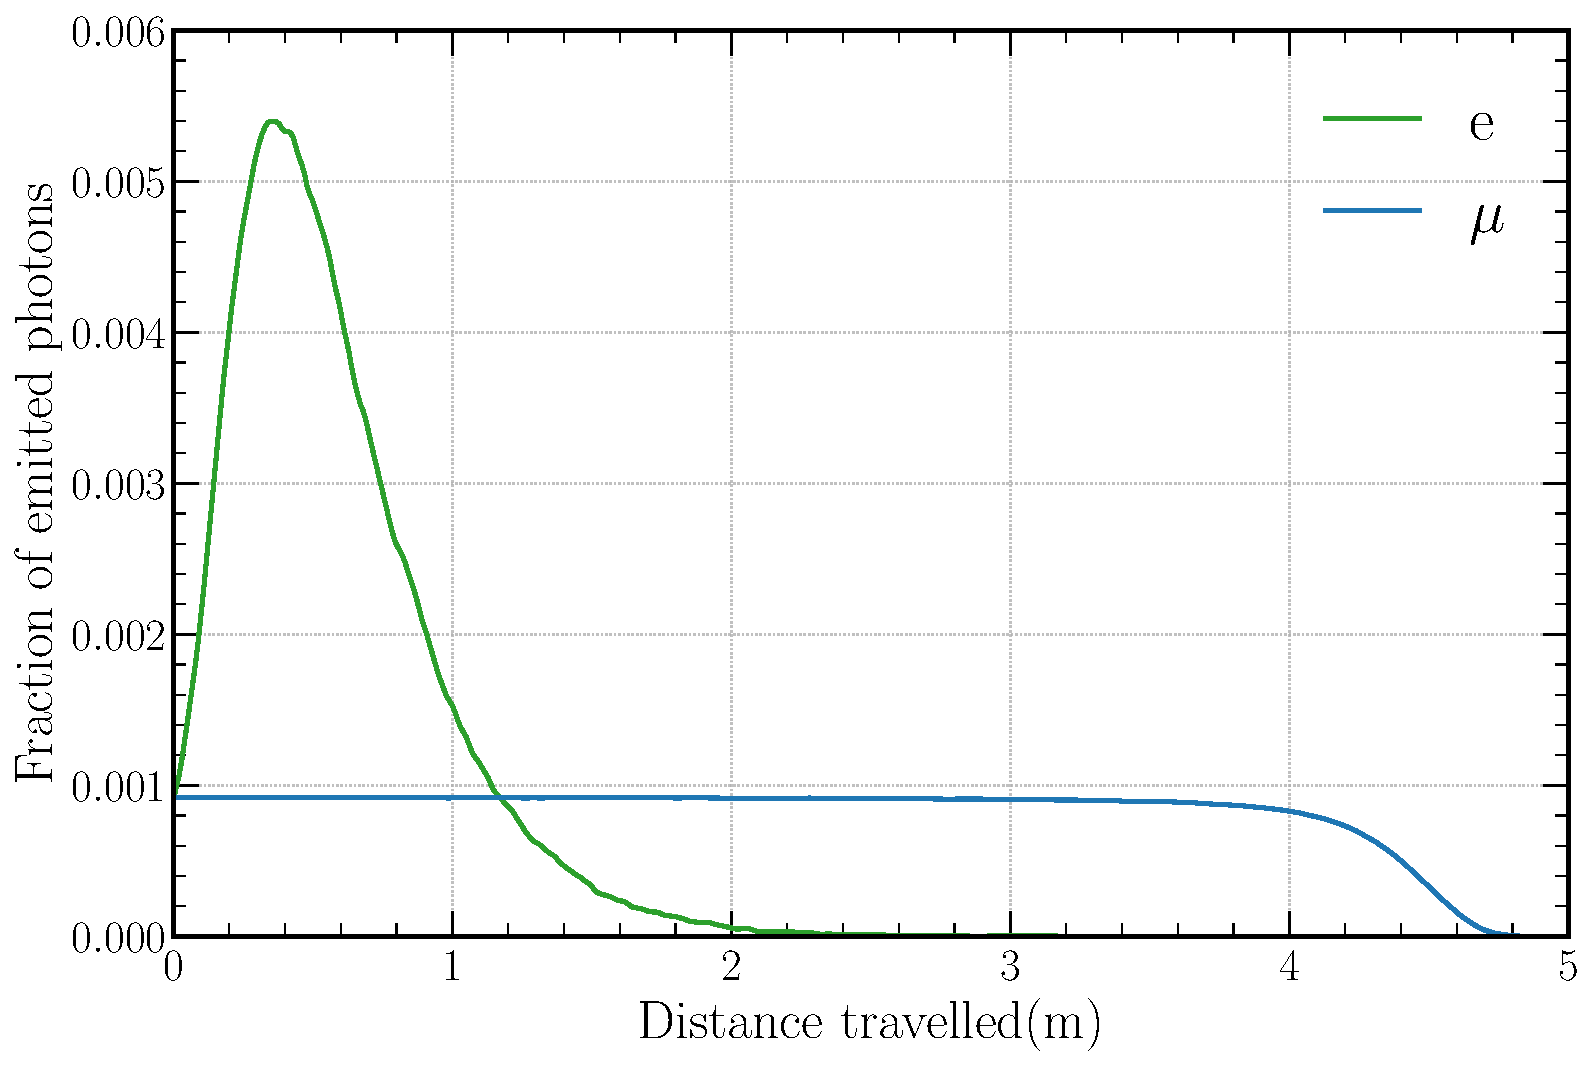
\includegraphics[width=0.6\textwidth]{diagrams/4-chips/emission_distance.pdf}
    \caption[Fraction of Cherenkov photons emitted as a function of distance.]
    {The fraction of the total number of photons emitted as a function of the distance from the
        interaction vertex for both electrons and muons with an energy of \unit{2.5}{\GeV}. Note
        how the muon travels much further emitted an approximately constant amount of Cherenkov
        radiation as it does so.}
    \label{fig:emission distance}
\end{figure}

The situation becomes more complicated when many charged particles above the Cherenkov threshold
are involved, which is typical at higher energies. In this case, multiple rings are observed,
which usually overlap, making reconstruction difficult. The worst-case scenario, however, is when
two rings entirely overlap, removing any ability to tell them apart. This is commonly the case for
NC interactions producing a $\pi^{0}$ in the final state, the primary background for CC $\nu_{e}$
appearance analyses after CC $\nu_{\mu}$ rejection.

With a 98.82\% branching ratio $\pi^{0}$ particles decay to a pair of photons~\cite{particle2020}.
Both photons like electrons almost immediately initiate an electromagnetic shower, leading to two
electron like rings. The separation angle between the ring is given by:
\begin{equation}
    (1-\cos\theta_{ij})=\frac{m_{\pi}^2}{2E_{i}E_{k}},
\end{equation}
where $m_{\pi}$ is the invariant mass of the $\pi^{0}$ and $E_{i}$ and $E_{j}$ are the energies of
the two photons respectively. Therefore, for a $\pi^{0}$ decaying to two \unit{1}{\GeV} photons,
there is just $\sim 8^{\circ}$ of separation between the rings, making them incredibly hard to
tell apart, especially when electron like rings are usually fuzzy. Additionally, if the two
photons have an unequal energy distribution, such that one is much more energetic, the dominant
photon ring can dominate and drown out the other, again leading to what looks like a single
electron ring.

\section{The \chipsfive detector} %%%%%%%%%%%%%%%%%%%%%%%%%%%%%%%%%%%%%%%%%%%%%%%%%%%%%%%%%%%%%%%%
\label{sec:chips_detector} %%%%%%%%%%%%%%%%%%%%%%%%%%%%%%%%%%%%%%%%%%%%%%%%%%%%%%%%%%%%%%%%%%%%%%%

- Will use this prototype detector to explain all the main detailed principles of a \chips
detector module. The chips-5 detector is the first of these units, at 25m in diameter and 12m
tall, leads to a fiducial volume of ~5kton. This detector will act as a proof of concept that the
R\&D has been a success and the provide possible improvements for future iterations.

- Wentworth Pit 2W in northern minnesota, disused and flooded surface Taconite ore (a type of iron
ore) mining pit, owned by Cliffs natural resources. 7 mrad off-axis of the \numi beam. Located at
a latitude of 47.58N and longitude of 92.13W. at a baseline of 712 km. Deep enough for ~50m of
overburden to reduce cosmic background. Advantages of heavy infrastructure for heavy industry,
power and roads. Polymet building less than mile from pit deployment site, can use as laboratory
for building and testing components. Water is drained from the pit in the spring to ensure it does
not overflow during the summer rainy season. Therefore, fluctuations of +-3m are expected over the
course of a year.

- Not at the ideal location (baseline) to measure the mass hierarchy in the \numi beam.
- Can help to constrain delta-cp by measuring electron neutrino appearance.
- Physics capabilities have been studied using GLoBES, should ask Tom for a nice plot and brief
description of how it all works.

\begin{figure} % PIT DIAGRAM %
    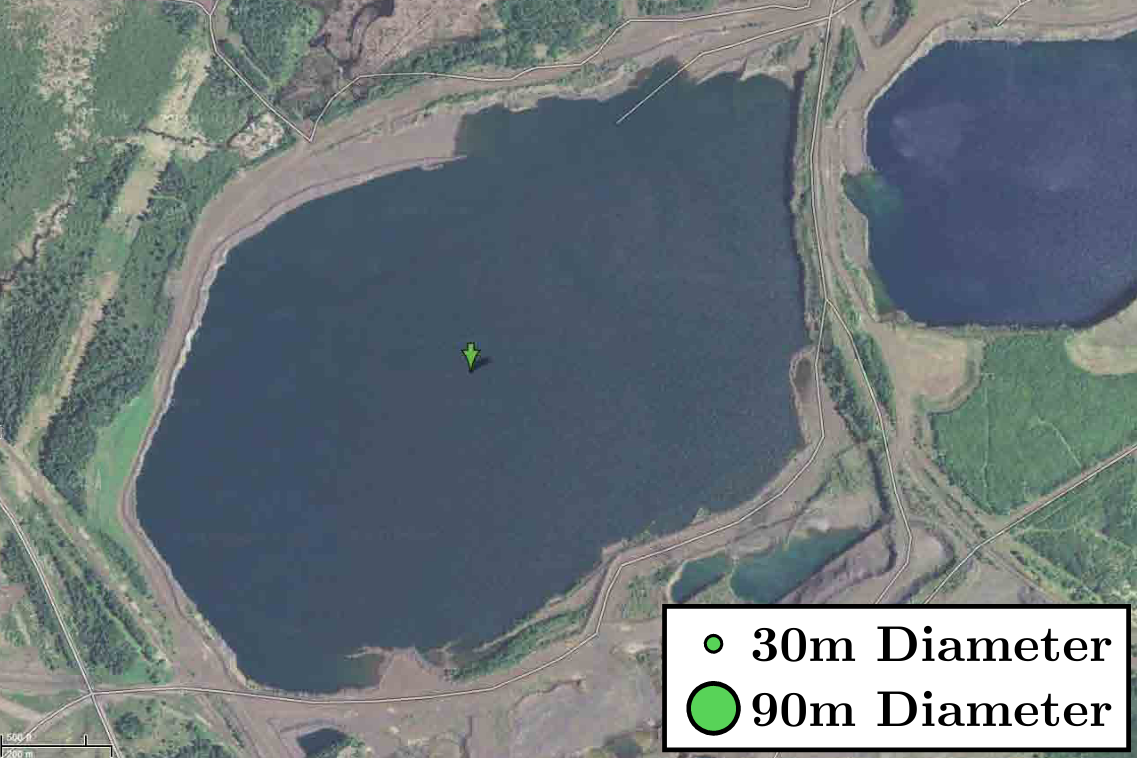
\includegraphics[width=0.6\textwidth]{diagrams/4-chips/location.png}
    \caption[Satellite view of the Wentworth 2W mine pit.]
    {Satellite view of the Wentworth 2W mine pit in northern Minnesota.
        The size markers are shown for scale. Image taken from Ref.\cite{adamson2013}.}
    \label{fig:location}
\end{figure}

\begin{figure} % PIT CONTOUR DIAGRAM %
    \includegraphics[width=0.6\textwidth]{diagrams/4-chips/contour_map.pdf}
    \caption[Topographic map of the Wentworth 2W mine pit.]
    {Topographic map of the Wentworth 2W mine pit. The contours are given in intervals of 5 feet,
        with the central areas of the pit having a depth of 50m. Image taken from
        Ref.\cite{adamson2013}.}
    \label{fig:contour_map}
\end{figure}

- A light tight liner a polymer membrane is used to separate the clean detector water from the
external pit water and isolate the detector volume.

INFO: detector module
- Dimensions
- Inner surface area
- PMT diameter
- photocathode coverage in different regions
- No of PMTs
- overburden
- CR muon rate
- In-spill CR occupancy
- CR event dead time
- Veto dimensions
- Veto num PMTs
- veto photocathode coverage
- veto pmt diameter

\begin{figure} % CHIPS RAMP DIAGRAM %
    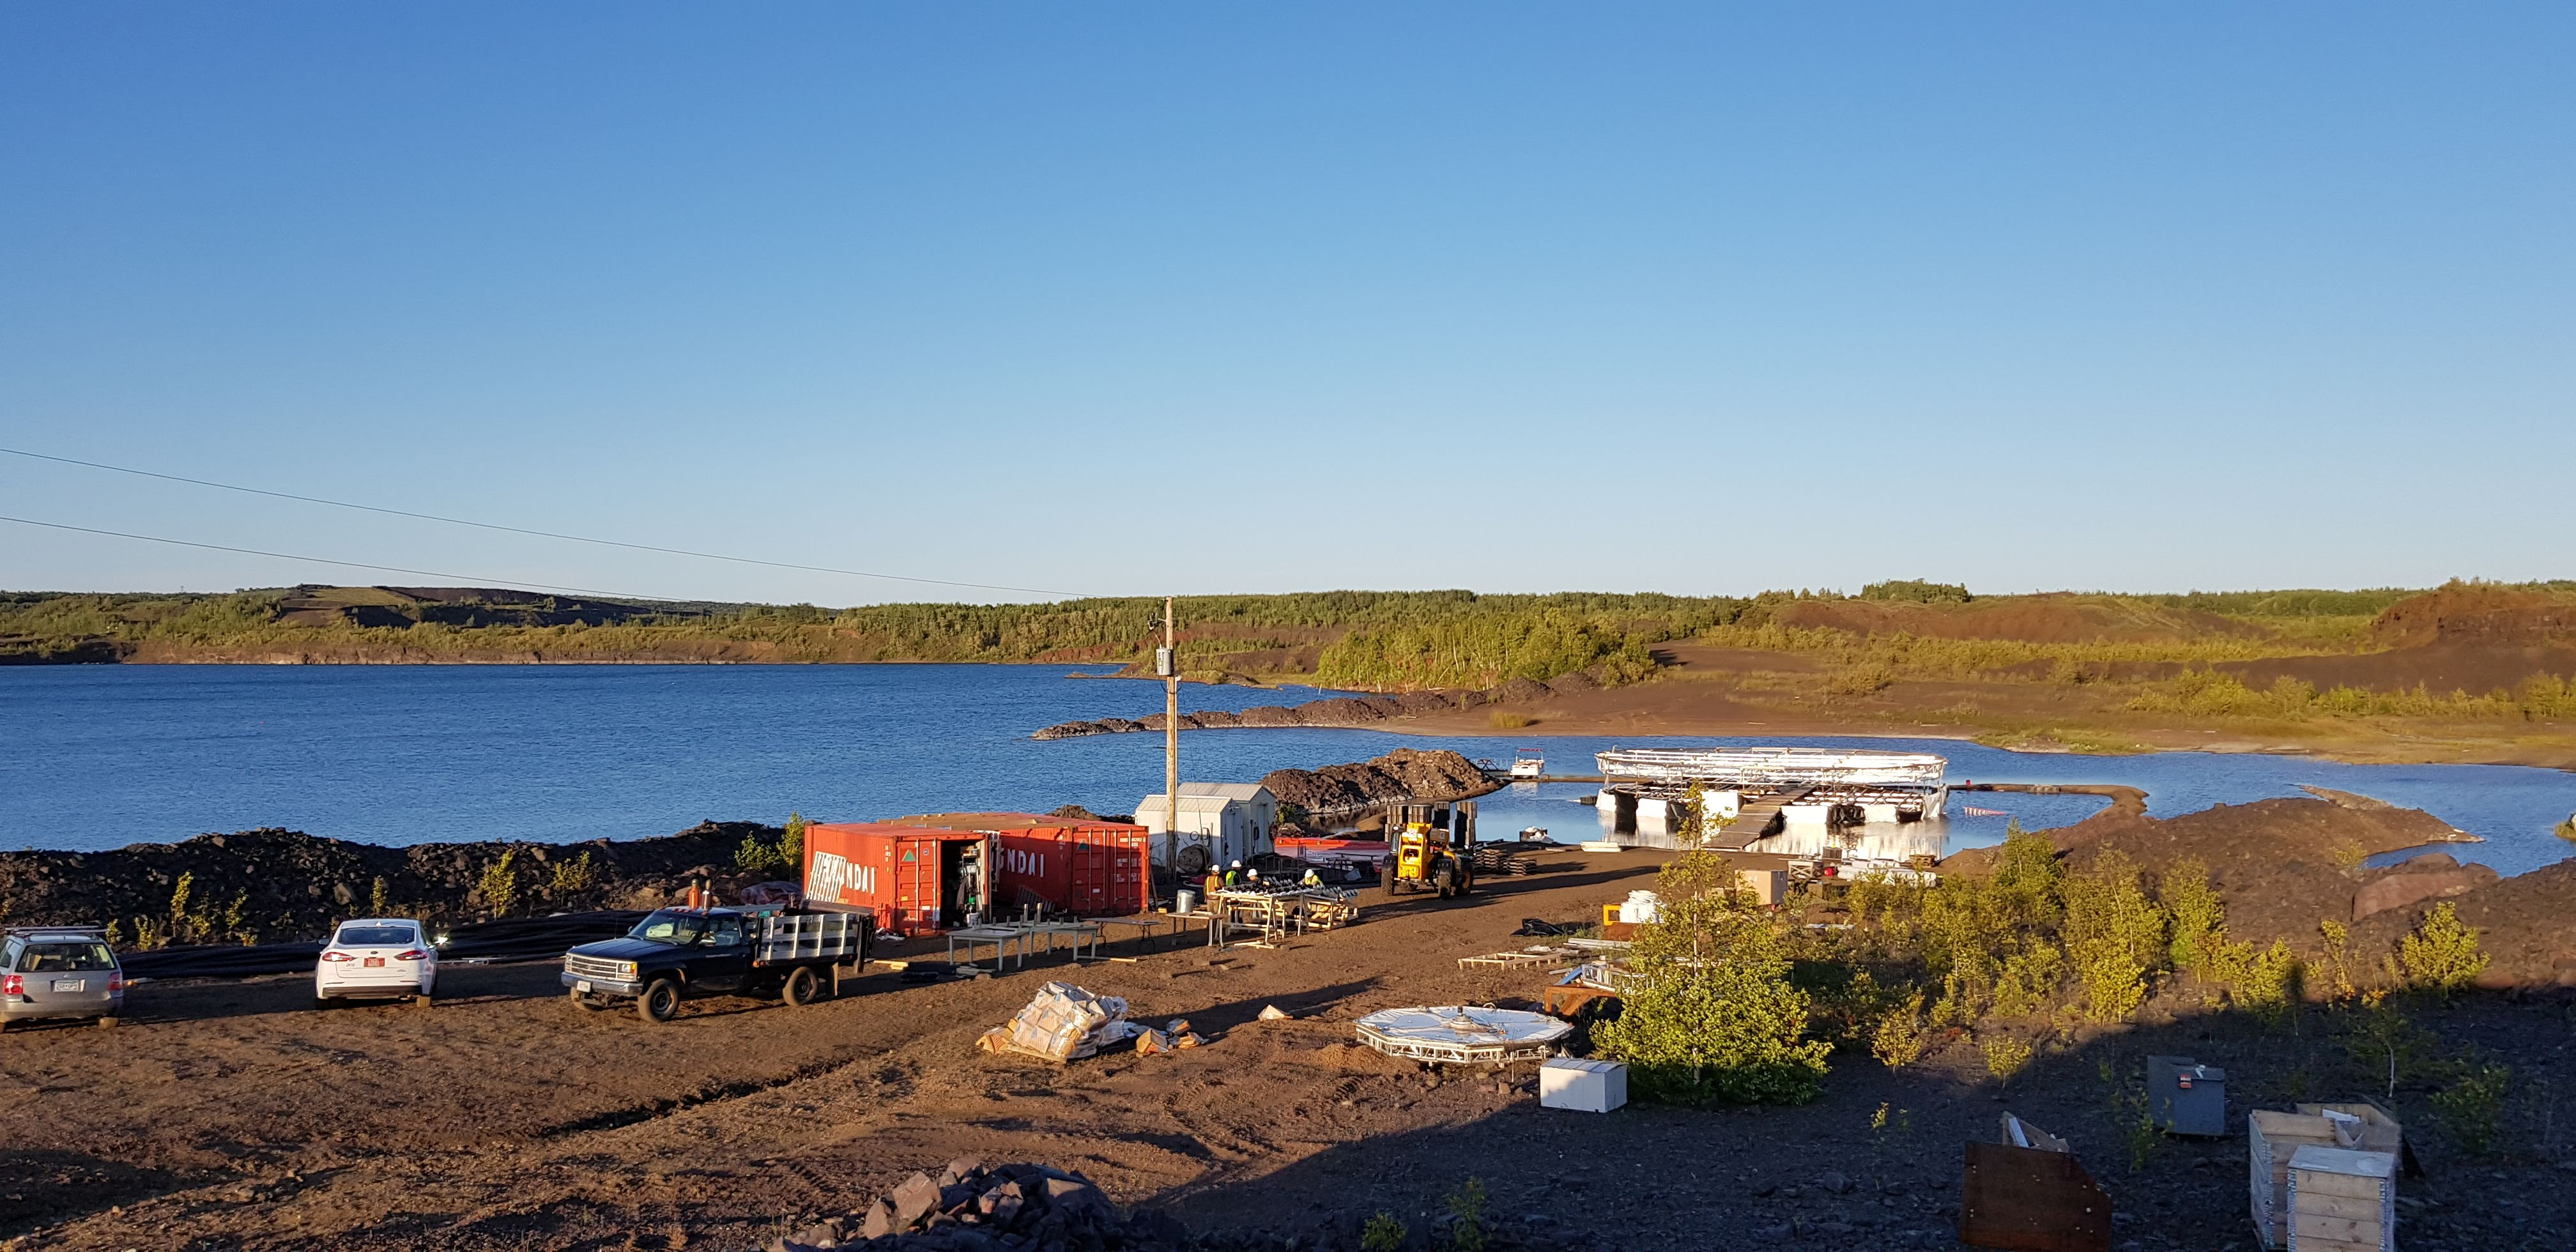
\includegraphics[width=\textwidth]{diagrams/4-chips/ramp.jpg}
    \caption[ramp.]
    {ramp.}
    \label{fig:ramp}
\end{figure}

\begin{figure} % CHIPS FROM THE SKY DIAGRAM %
    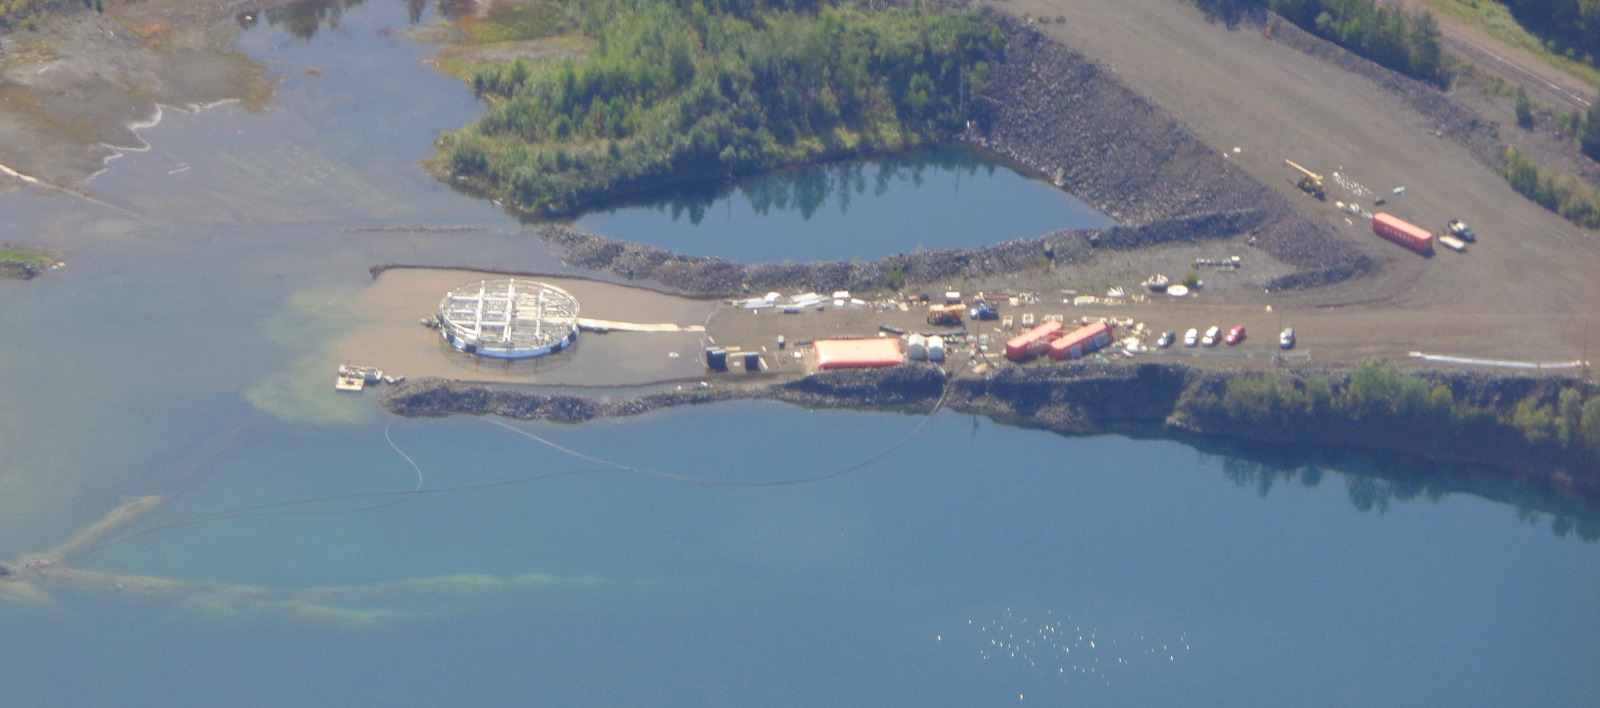
\includegraphics[width=\textwidth]{diagrams/4-chips/from_the_sky.jpg}
    \caption[Picture of the \chips detector from the air.]
    {Picture of the \chips detector taken from an airplane. The Wentworth 2W pit is in the lower
        half of the image, with the half built detector, huts and construction containers
        visable.}
    \label{fig:from_the_sky}
\end{figure}

\subsection{Structure} %%%%%%%%%%%%%%%%%%%%%%%%%%%%%%%%%%%%%%%%%%%%%%%%%%%%%%%%%%%%%%%%%%%%%%%%%%%
\label{sec:chips_detector_structure} %%%%%%%%%%%%%%%%%%%%%%%%%%%%%%%%%%%%%%%%%%%%%%%%%%%%%%%%%%%%%

\begin{figure} % CHIPS SUNRISE DIAGRAM %
    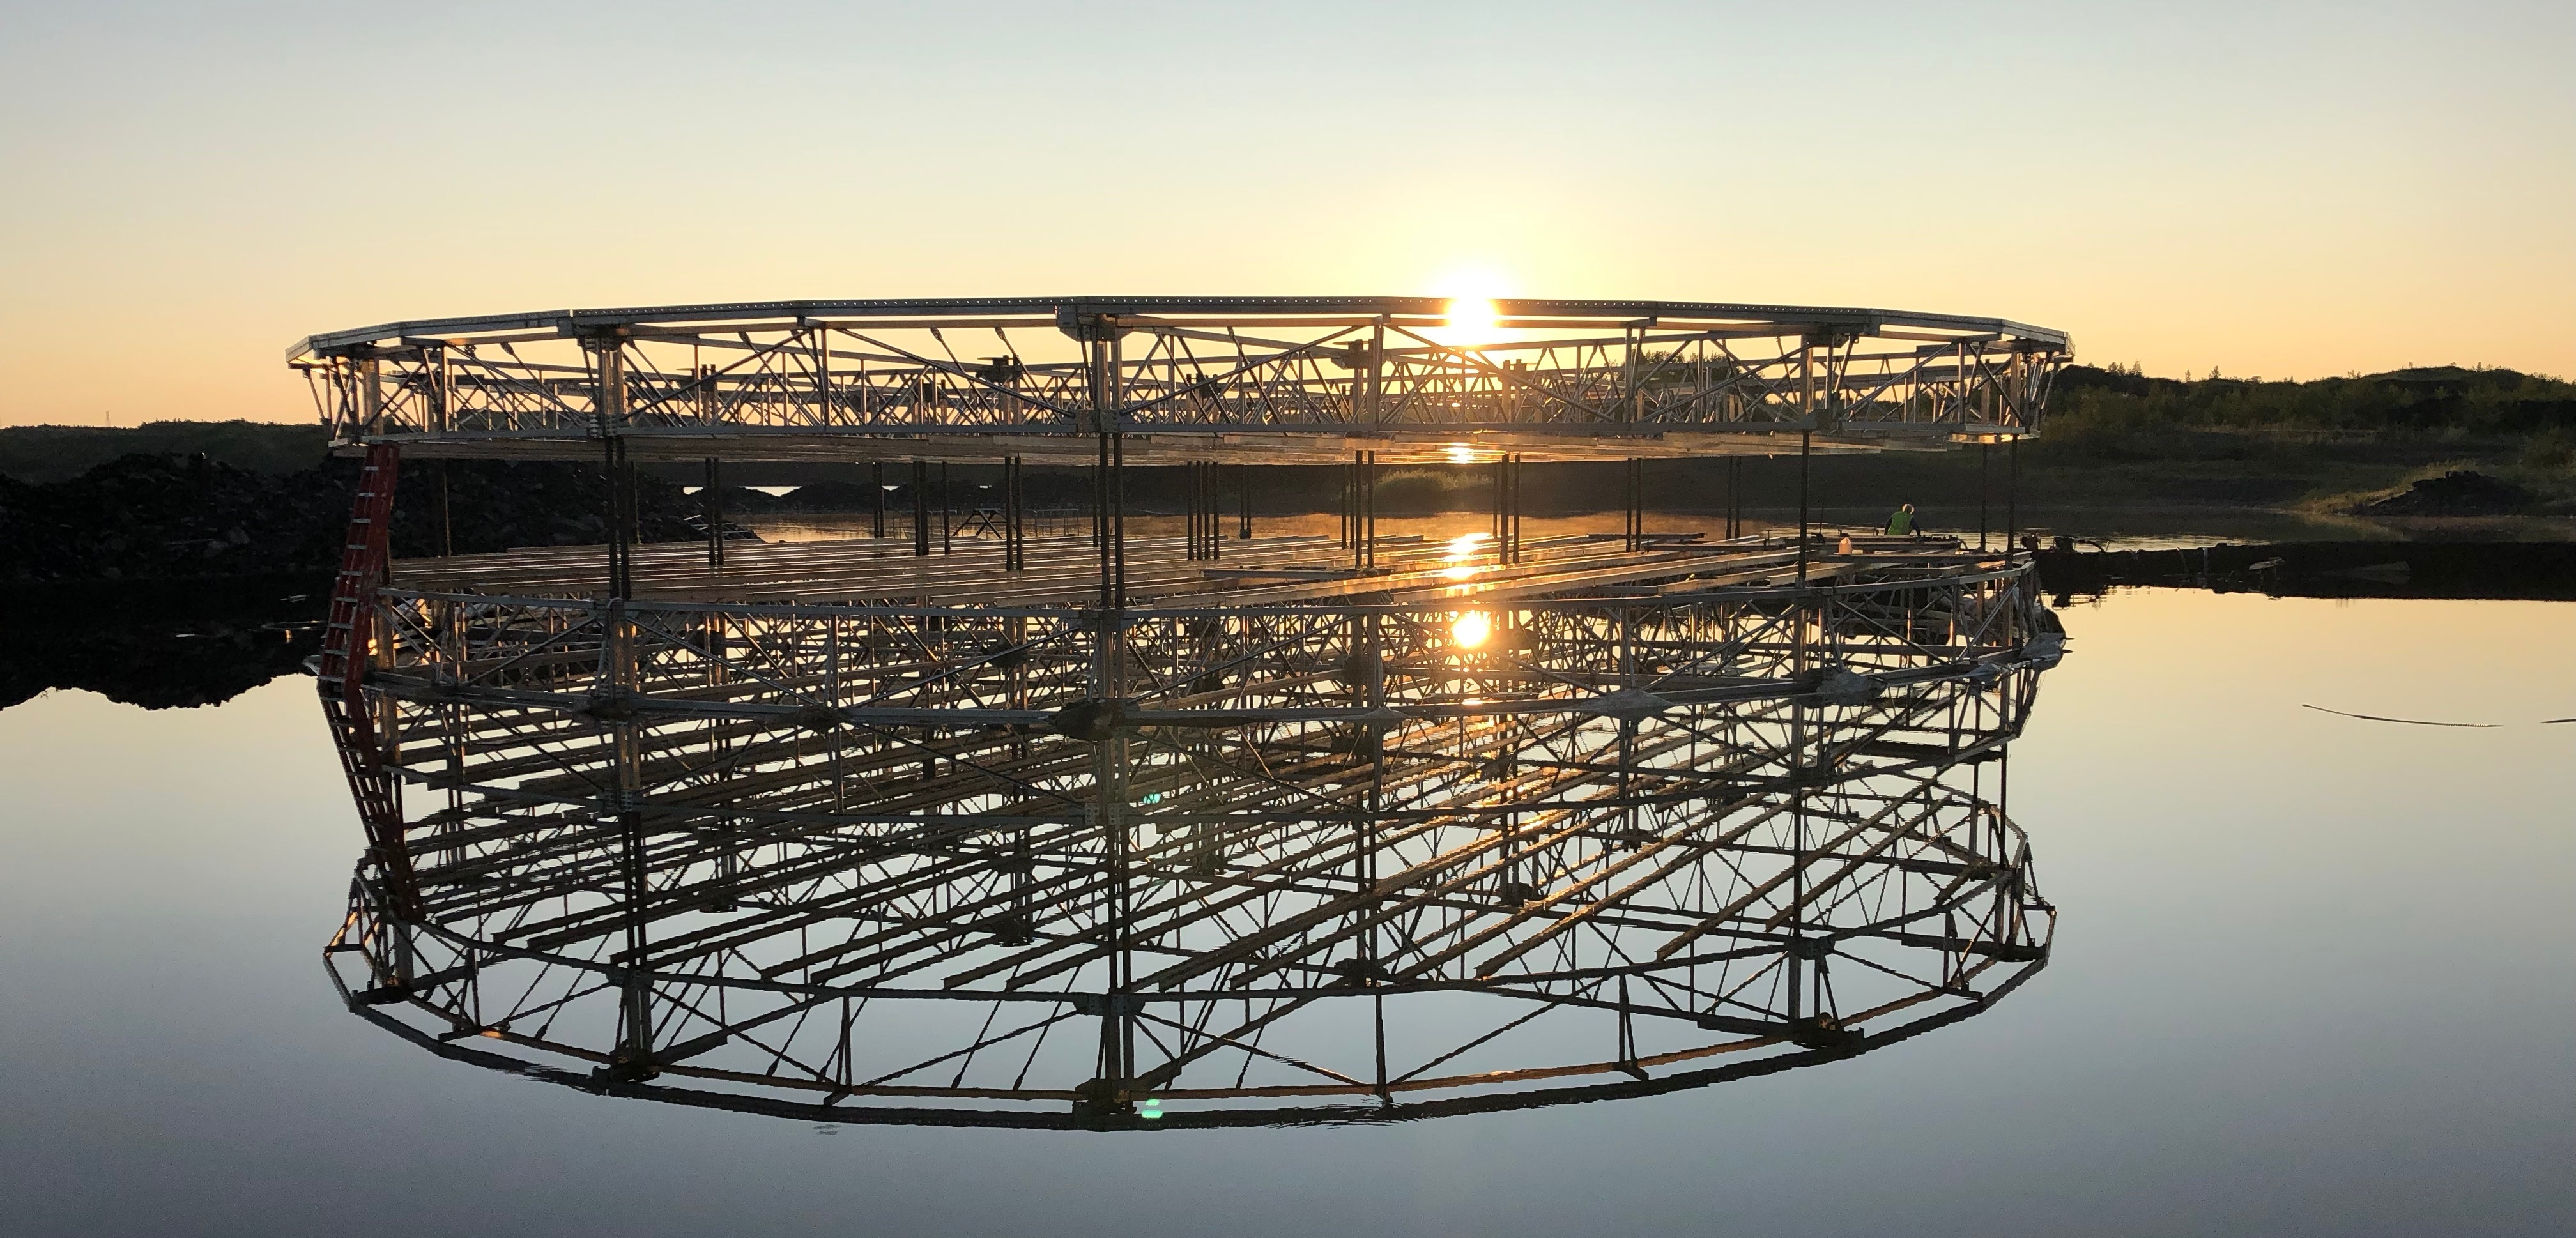
\includegraphics[width=\textwidth]{diagrams/4-chips/sunrise_short.jpeg}
    \caption[Sunrise over the \chips detector.]
    {Sunrise over the \chips detector structure. The perfectly calm pit water
        produces the mirror effect.}
    \label{fig:sunrise}
\end{figure}

\begin{figure} % CHIPS RENDER 1 DIAGRAM %
    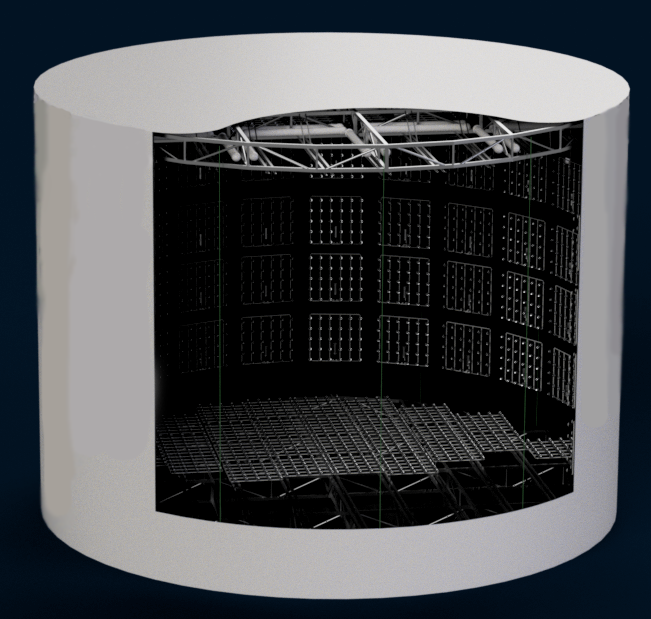
\includegraphics[width=0.6\textwidth]{diagrams/4-chips/chips_render_1.png}
    \caption[Graphical rendering of the \chipsfive detector with liner cutaway.]
    {Graphical rendering of the \chipsfive detector with a section of the liner cutaway.
        The bottom endcap and wall planes are visable,
        as well as the top endcap structure and floatation.}
    \label{fig:chips_render_1}
\end{figure}

\begin{figure} % CHIPS RENDER 2 DIAGRAM %
    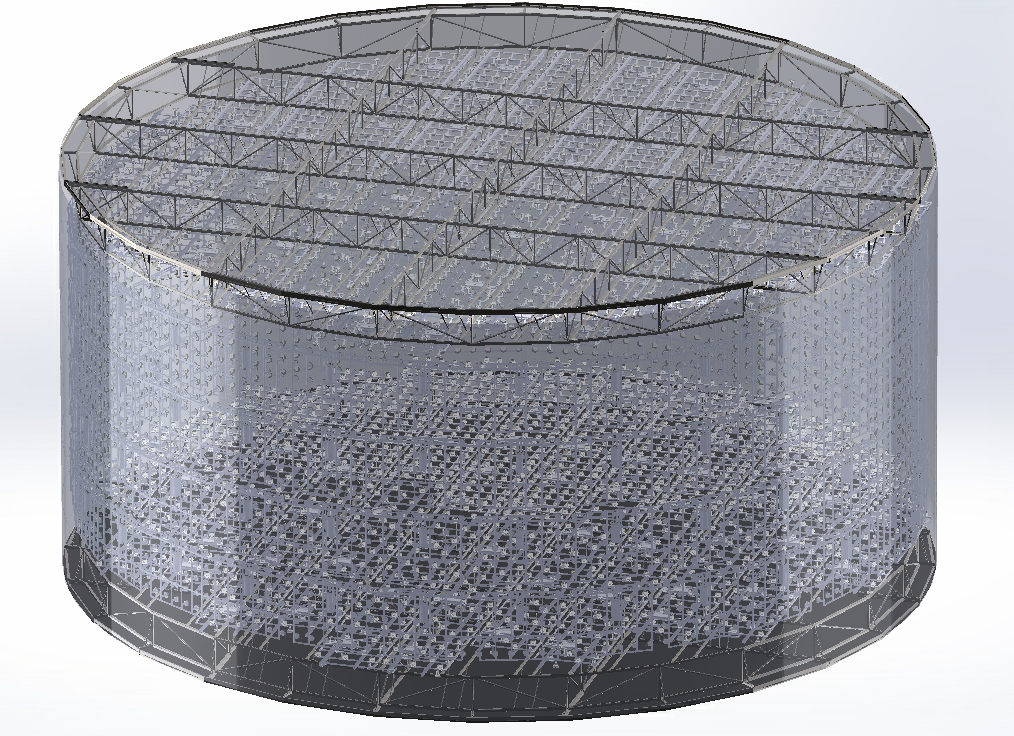
\includegraphics[width=0.6\textwidth]{diagrams/4-chips/chips_render_2.png}
    \caption[Graphical rendering of the \chipsfive detector structure.]
    {Graphical rendering of the \chipsfive detector structure.}
    \label{fig:chips_render_2}
\end{figure}

\subsection{Instrumentation} %%%%%%%%%%%%%%%%%%%%%%%%%%%%%%%%%%%%%%%%%%%%%%%%%%%%%%%%%%%%%%%%%%%%%
\label{sec:chips_detector_instrumentation} %%%%%%%%%%%%%%%%%%%%%%%%%%%%%%%%%%%%%%%%%%%%%%%%%%%%%%%

km3net 2.0 ref in \cite{adrian2016}
Icecube DOM paper \cite{hanson2006}

DIAGRAM: POM diagram
REF: Km3net optical module paper
REF: Nemo-3 PMT paper
- CHIPS uses high quantum efficiency PMTs from Hamamatsu
REF: Get hamamatsu PMT reference
- We will talk in detail about DAQ in the following chapter
- For calibration "flashers" are built into the detector to allow for known location light
generation to calibrate final PMT positions and time resolutuions.

\begin{figure} % PMT ASSEMBLY DIAGRAM %
    \centering
    \subcaptionbox{pmt disassembled\label{fig:pmt_disassembled}}{%
        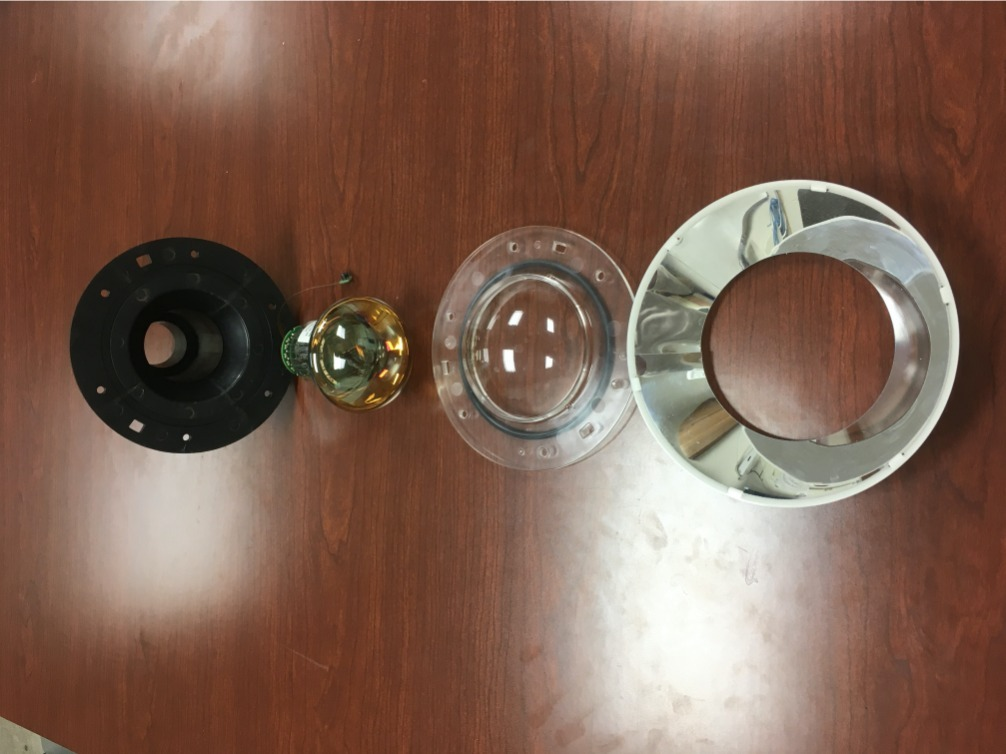
\includegraphics[height=5cm]{diagrams/4-chips/pmt_disassembled.jpg}%
    }
    \quad
    \subcaptionbox{pmt assembled\label{fig:pmt_assembled}}{%
        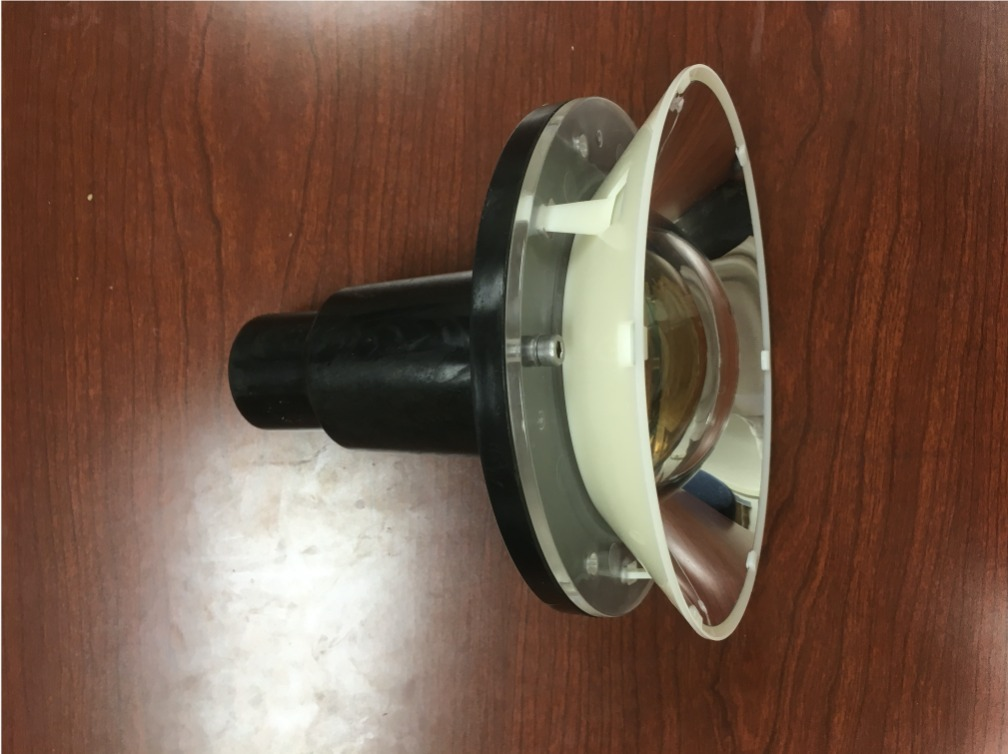
\includegraphics[height=5cm]{diagrams/4-chips/pmt_assembled.jpg}%
    }
    \caption[The caption]
    {The caption}
\end{figure}

\begin{figure} % NIKHEF PLANE DIAGRAM %
    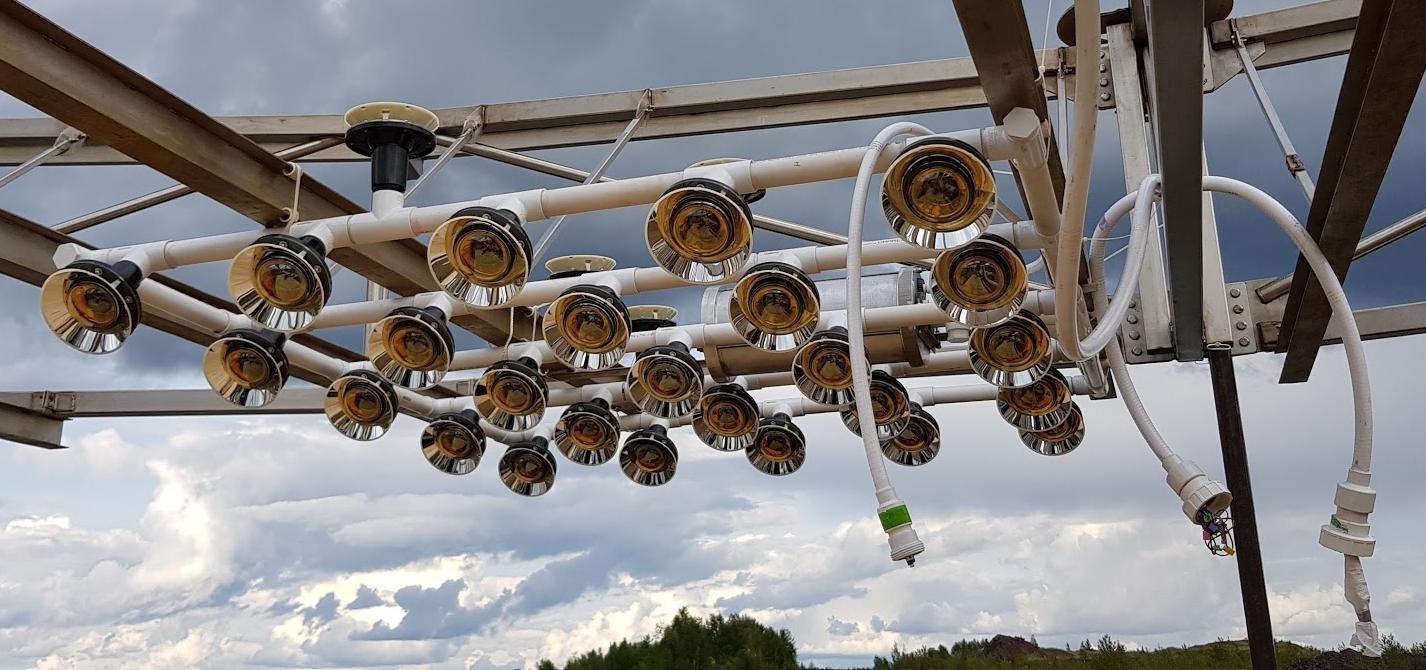
\includegraphics[width=\textwidth]{diagrams/4-chips/single_plane.jpg}
    \caption[Picture of a single `Nikhef' plane.]
    {Picture of a single `Nikhef' high density top endcap plane. Both the inward facing and veto
        PMTs can be seen as well as the planes umbilical with the green tape attached.}
    \label{fig:single_plane}
\end{figure}

\subsection{Water clarity} %%%%%%%%%%%%%%%%%%%%%%%%%%%%%%%%%%%%%%%%%%%%%%%%%%%%%%%%%%%%%%%%%%%%%%%
\label{sec:chips_detector_water} %%%%%%%%%%%%%%%%%%%%%%%%%%%%%%%%%%%%%%%%%%%%%%%%%%%%%%%%%%%%%%%%%

- Though remarkably clear the Wentworth pit water is not clean enough for the detector volume
where we require ~30m attenuation length.

\subsection{Deployment} %%%%%%%%%%%%%%%%%%%%%%%%%%%%%%%%%%%%%%%%%%%%%%%%%%%%%%%%%%%%%%%%%%%%%%%%%%
\label{sec:chips_detector_deployment} %%%%%%%%%%%%%%%%%%%%%%%%%%%%%%%%%%%%%%%%%%%%%%%%%%%%%%%%%%%%

DIAGRAM: Floating dock diagram
DIAGRAM: Deployment diagram
- How it can grow if needed

\subsection{Current status} %%%%%%%%%%%%%%%%%%%%%%%%%%%%%%%%%%%%%%%%%%%%%%%%%%%%%%%%%%%%%%%%%%%%%%
\label{sec:chips_detector_status} %%%%%%%%%%%%%%%%%%%%%%%%%%%%%%%%%%%%%%%%%%%%%%%%%%%%%%%%%%%%%%%%

\section{Monte Carlo event generation and simulation} %%%%%%%%%%%%%%%%%%%%%%%%%%%%%%%%%%%%%%%%%%%%
\label{sec:chips_monte_carlo} %%%%%%%%%%%%%%%%%%%%%%%%%%%%%%%%%%%%%%%%%%%%%%%%%%%%%%%%%%%%%%%%%%%%

\subsection{Beam event generation} %%%%%%%%%%%%%%%%%%%%%%%%%%%%%%%%%%%%%%%%%%%%%%%%%%%%%%%%%%%%%%%
\label{sec:chips_monte_carlo_beam} %%%%%%%%%%%%%%%%%%%%%%%%%%%%%%%%%%%%%%%%%%%%%%%%%%%%%%%%%%%%%%%

\begin{figure} % CHIPS FLUX DIAGRAM %
    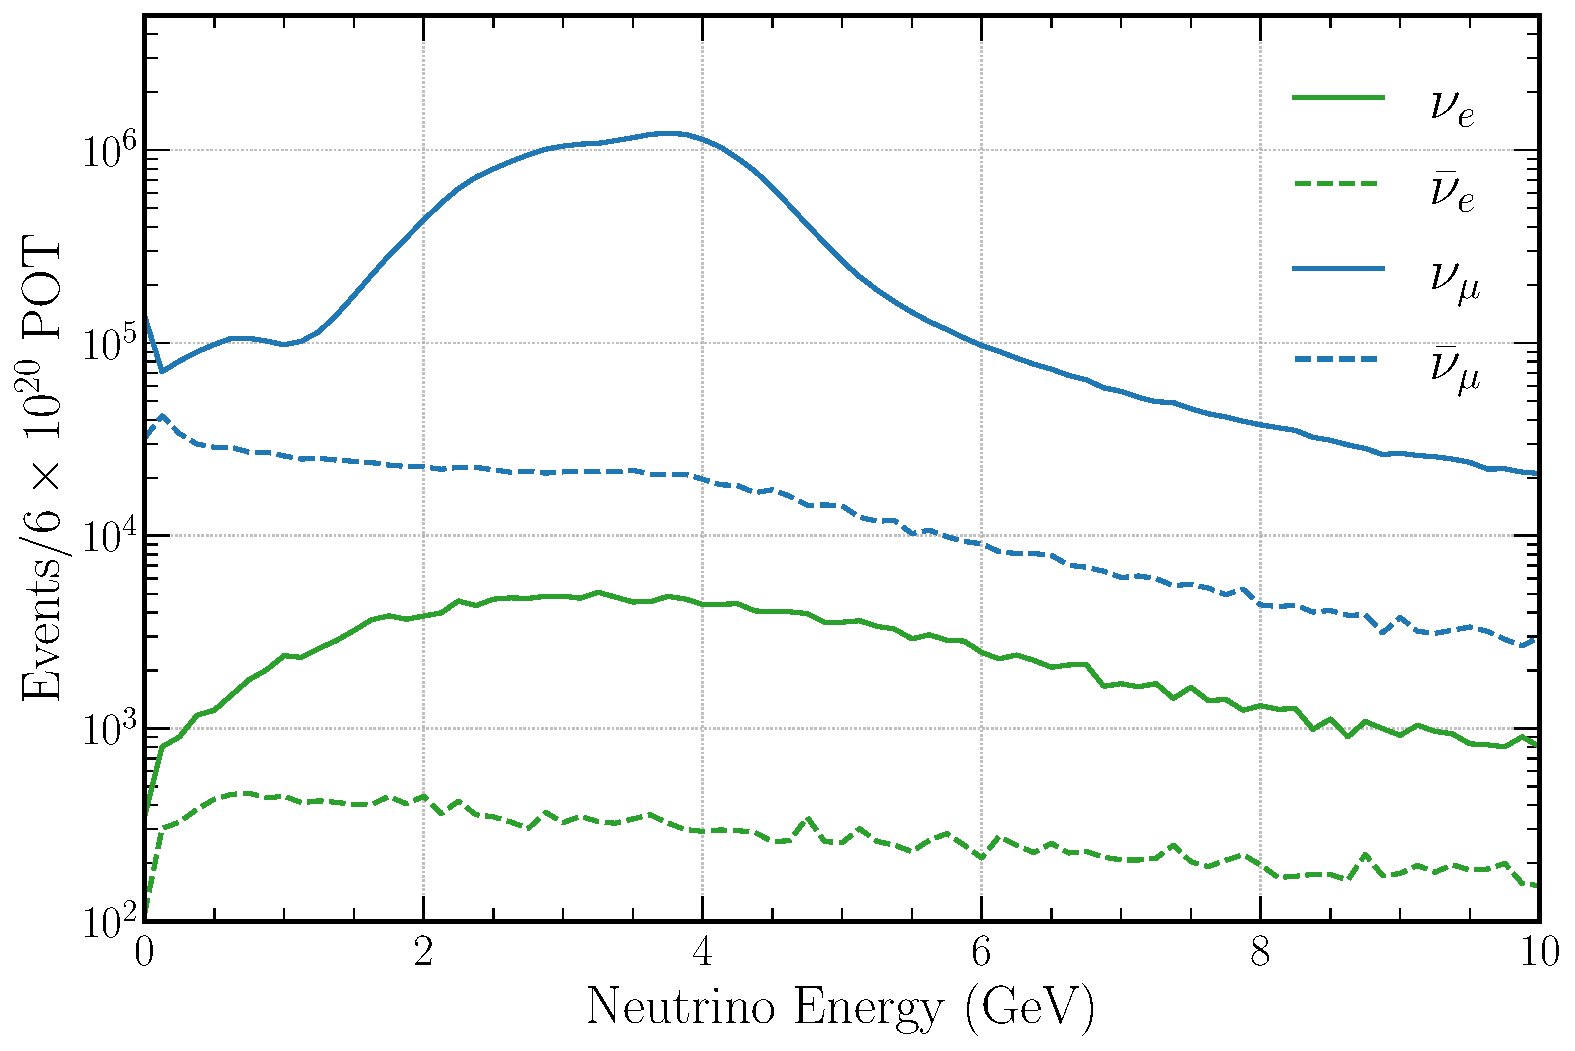
\includegraphics[width=0.8\textwidth]{diagrams/4-chips/flux.pdf}
    \caption[\numi neutrino flux at CHIPS.]
    {The \numi beam neutrino flux with cross-sections applied at the CHIPS detector location. Shown
        are the seperate contributions from the different neutrino types and sign. No oscillations
        have been applied.}
    \label{fig:flux}
\end{figure}

- Cosmic event rate in \cite{son2013}

- We take full advantage of the MINOS, \nova extensive simulations of the \numi beam for use in
CHIPS.
- The tau neutrino component is negligible and not predicted by the simulation
INFO: expected number of events per year etc...

\subsection{Cosmic event generation} %%%%%%%%%%%%%%%%%%%%%%%%%%%%%%%%%%%%%%%%%%%%%%%%%%%%%%%%%%%%%
\label{sec:chips_monte_carlo_cosmic} %%%%%%%%%%%%%%%%%%%%%%%%%%%%%%%%%%%%%%%%%%%%%%%%%%%%%%%%%%%%%

DIAGRAM: expected cosmic rate at different height plot
DIAGRAM: Cosmic rate given the water overburden diagram

- These short spills are essential for \chips and other experiments in rejecting the massive
cosmic ray background. As all events outside the expected beam spill window at the detector can be
rejected.

\begin{figure} % COSMICS AROUND DETECTOR DIAGRAM %
    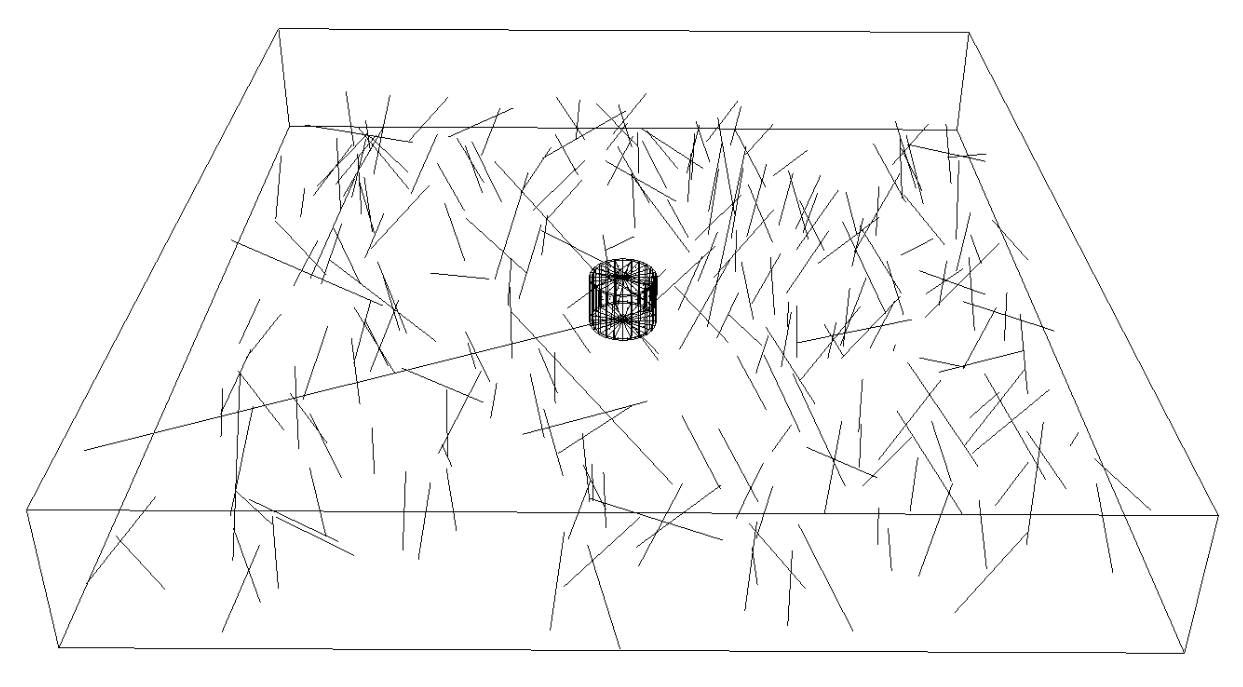
\includegraphics[width=0.8\textwidth]{diagrams/4-chips/cosmics.png}
    \caption[Cosmic muon rays around the CHIPS detector]
    {Simulated cosmic muon rays around the CHIPS detector. Note how they are generated within a
        box.}
    \label{fig:cosmics}
\end{figure}

\subsection{Detector simulation} %%%%%%%%%%%%%%%%%%%%%%%%%%%%%%%%%%%%%%%%%%%%%%%%%%%%%%%%%%%%%%%%%
\label{sec:chips_monte_carlo_sim} %%%%%%%%%%%%%%%%%%%%%%%%%%%%%%%%%%%%%%%%%%%%%%%%%%%%%%%%%%%%%%%%

\begin{figure} % SIMULATED EVENT DISPLAY DIAGRAM %
    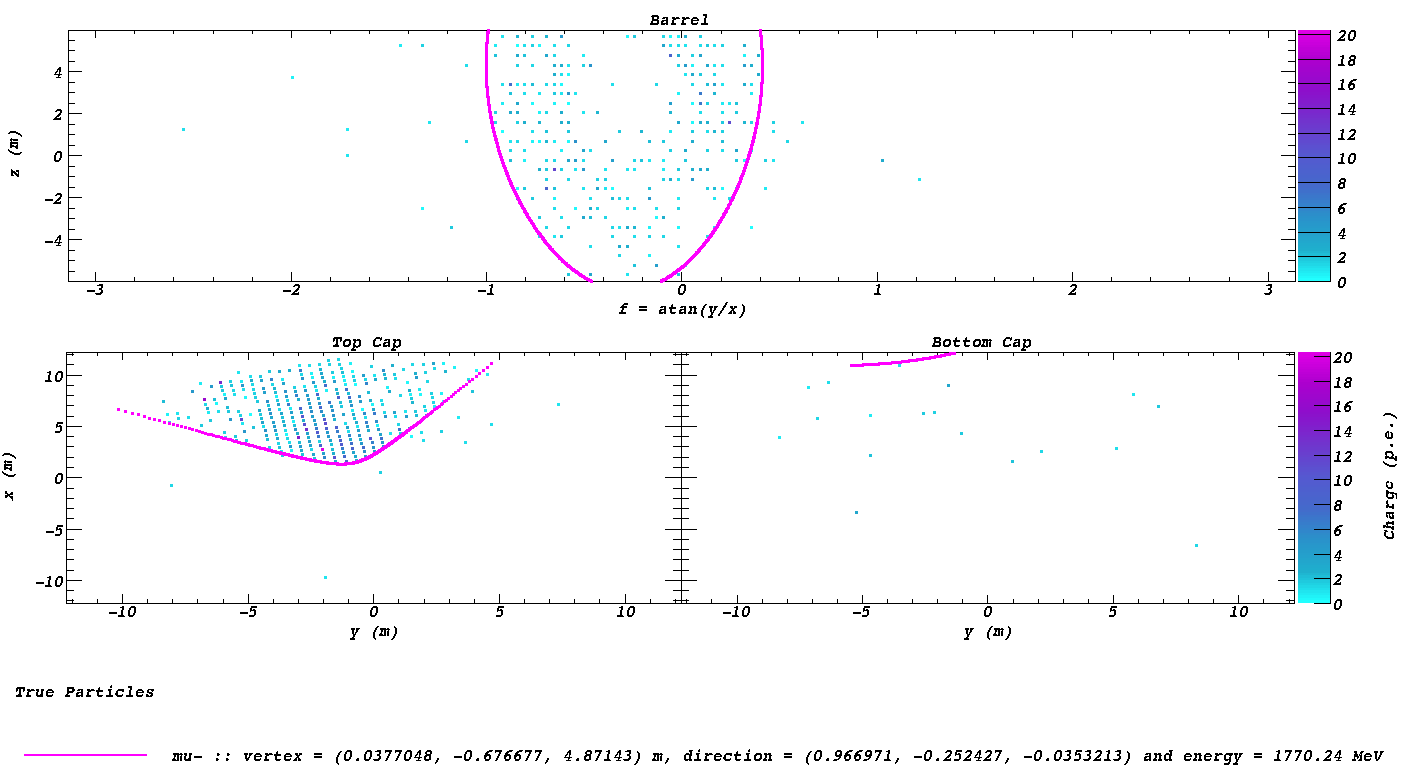
\includegraphics[width=\textwidth]{diagrams/4-chips/sim_event.png}
    \caption[sim event short]
    {$\nu_{\mu}$ CC quasi-elastic event with a single muon final state particle of energy
        1770.24 MeV}
    \label{fig:sim_event}
\end{figure}

\begin{figure} % DIGI DIAGRAM %
    \centering
    \subcaptionbox{\label{fig:digi_method}}{%
        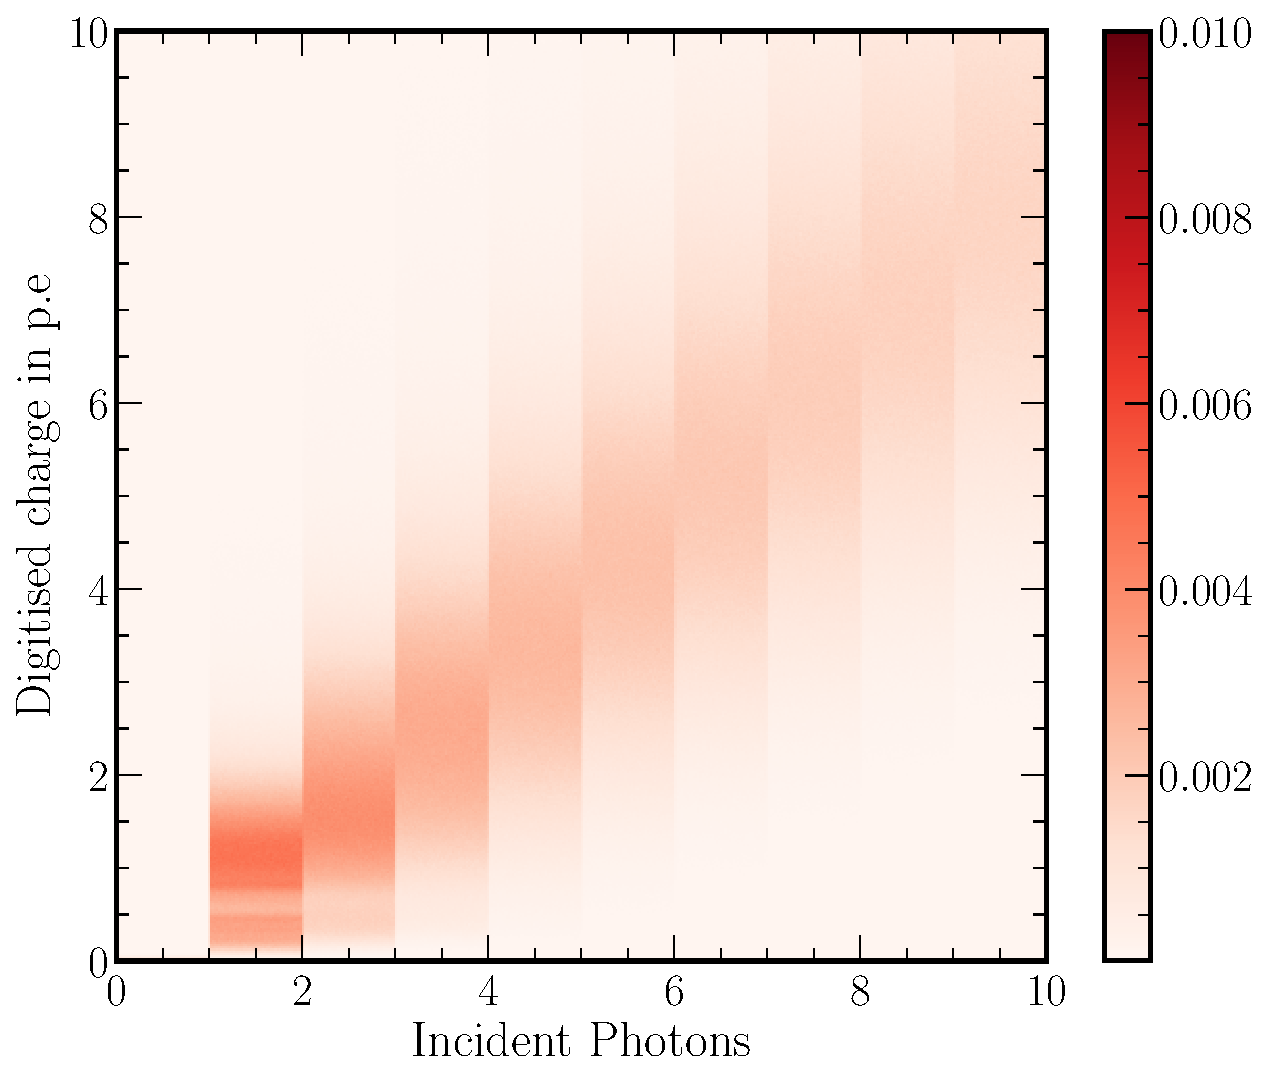
\includegraphics[height=6cm]{diagrams/4-chips/digi_method.pdf}%
    }
    \quad
    \subcaptionbox{\label{fig:digi_likelihood}}{%
        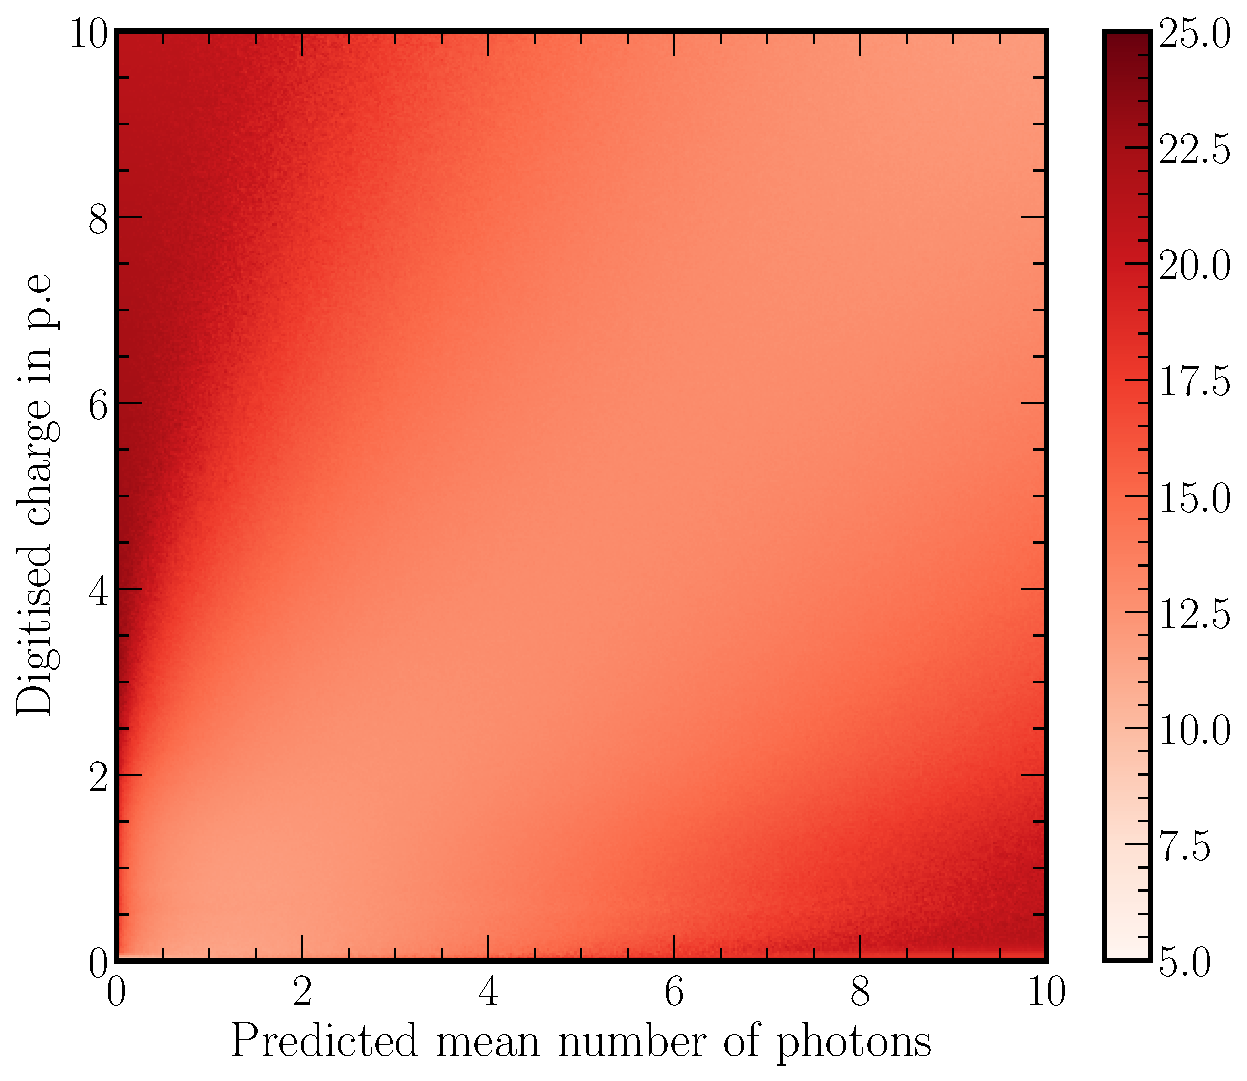
\includegraphics[height=6cm]{diagrams/4-chips/digi_likelihood.pdf}%
    }
    \caption[Simulation PMT digitisaion function.]
    {(a) Digitisation function used within the simulation to convert incident photons to measured
        digitised charge. (b) Likelihood of a measured digitised charge being caused by a number
        of photons incident on a PMT.}
    \label{fig:digitisation}
\end{figure}

- The "signal" in all cases are CC interactions, therefore selection of nuel, anuel, numu and
anumu CC is the goal.
- Main background in CC numu selections are NC with charged pions.
- Main background in CC nuel selections is pi-zero NC, which can mimic the chracteristic EM
shower, due to its near certain decay into two photons.
- You get a small number of nuel intrinsic to the beam, they are just a background as they are
indistinguishabe from the nuel appreaence neutrinos.
- Once you have collected samples in all four cases, a fit is performed to the reconstructed
neutrino energy distributions to extract the four neutrino oscillation parameters.